\begin{htmlonly}


\usepackage{html, htmllist}
\usepackage{longtable}

\bodytext{bgcolor="#ffffff" link="#0033cc" vlink="#0033cc"}

%%%==================================================	
%%%==================================================	

% #1  mark defined by \label
% #2  a linktext 
% #3  a html link 
\newcommand{covlink}[3]{\htmladdnormallink{#2}{#3} \latex{(\ref{#1})} }


\newenvironment{covimg}[4]%
{
 \begin{figure}[htp]
  \begin{center}
   \latexonly
      \includegraphics[scale=#4]{#1/pict/#2}
   \endlatexonly  
   \html{\htmladdimg[align="center"]{pict/#2.png}}
   \caption{#3}
  \end{center}
 \end{figure} 
}{} 

\newenvironment{covimg2}[3]%
{ 
 \begin{figure}[htp]
  \begin{center}
     \latexonly
       \includegraphics[scale=#3]{#1/pict/#2}   
     \endlatexonly
     \html{\htmladdimg[align="center"]{pict/#2.png}}
  \end{center}
 \end{figure} 
}{}

\definecolor{output}{rgb}{0.,0.,1.}
\definecolor{depend}{rgb}{1.,0.65,0.}
\definecolor{required}{rgb}{0.58,0.,0.83}
\definecolor{optional}{rgb}{0.,0.39,0.}

\newcommand{\addimage}[1] {\html{\htmladdimg{pict/#1.png}}}

\newcommand{\addpict}[4] {\latexonly
	     \begin{figure}[!htbp]
			  \begin{center}
   	 		  \includegraphics[scale=#1]{#2}
   	 		  \caption{#3}
		 		  \label{#4}
			  \end{center}
	 		\end{figure}
	     \endlatexonly}



\newcommand{\mapeditor}{\textbf{Map Editor}}
\newcommand{\covise}{\textbf{COVISE}}


\end{htmlonly}



%=============================================================
%=============================================================

\startdocument
\chapter{The Renderer}
\label{Renderer}

\section{Introduction}

In this chapter the main functionality of the COVISE Renderer is summarized.
Like the map editor, one renderer is started on every host in a cooperative
working session, once the master renderer has been brought up on the master map editor. 

The design of the Renderer supports collaborative working (for more details see chapter 5,
COVISE CE - Collaborative Working): Basically the Renderer works in a 
"what you see is what I see" mode. This is called
the Master/Slave Mode or Tight Coupling. It means, that every partner in the session
has the same viewpoint in respect to the rendered geometry objects. Only the 
master has the ability to change the view in the other renderers. On the slave
side it is possible to change the camera position independently from the others
as long as the master isn't changing anything. As soon as the master performs an
interaction, the slaves automatically become synchronized and updated.
(Strictly speaking, there is a
slight difference between "Master/Slave Mode" and "Tight Coupling": "Master/Slave" causes the slave
renderer to be updated at the end of a move only, whereas "Tight" makes a contiuous update. The two
possibilities have been introduced due to performance considerations.) 

Alternatively, the master has the ability to switch to a second mode called Loose
Coupled Mode. When this mode is enabled, every partner has full access to all
Renderer functionalities without disturbing the other partners setup and view.
This mode is convenient when the partners have stopped their discussion about the
current rendered objects and want to do some postprocessing on the data, like
changing some colors, adding light sources, saving or printing etc.. 

The discussion on the data is supported by introducing Telepointers. A telepointer
marks a position in the renderer's window to guide the other partners to interesting
details on the screen. Each renderer has a telepointer attached to the current
mouse position, which is sent to the remote renderers.

In addition, the renderer supports stereo viewing mode with the Crystal Eyes
shutter glasses as well as with various autostereoscopic viewing devices.
It also supports the Spaceball or the DLR Spacemouse for 6Degree of Freedom interaction.

\section{Getting started}
To start the Renderer simply select the module named Renderer in
the category Renderer in the MapEditor. After a few moments the renderer's icon \ref{fig48}
is displayed in the MapEditor canvas and the renderer main window appears on the
screen as shown in \ref{fig50}.

 \html{\htmladdimg{pict/image1.png}} 
 \latexonly
 \begin{figure}[htp]
  \begin{center}
   
\includegraphics[scale=0.7]{renderer/pict/image1}
   \caption{The Renderer Icon}
	\label{fig48}
  \end{center}
 \end{figure}
 \endlatexonly

Note that you can resize the renderer according to your needs, but reducing the
window size may hide some of the menu components. By clicking on the module setup
button in the Renderer icon, the data object and parameter list for the Renderer
appears (\ref{fig49}).

As you can see, no parameters can be set or adjusted, and there is currently only
one input port called DO\_Geometry. In the future there may be additional input
ports, e.g. for pixel images. Unlike other application modules in the COVISE
environment, the renderer has it's own Motif based point and click user interface.
You can connect all modules with geometry output ports to the renderer's input
port. The renderer will accept any number of input objects. After an execution
of a complete module network, the renderer will appear highlighted while new
objects from local memory or remote machines are sent into the module. New
rendered objects will be shown in the geometry objects list in full name. You
can find out your point of view in respect to the scene by looking at the
coordinate axes and their orientation. If you cannot see objects just select
the View All icon on the right side of the drawing area. 

You see the objects as you would look through a camera lens. While pressing
the left mouse button and dragging the mouse around in the Viewer Area, you
can move the camera around the scene. This allows you to rotate the whole view
around a point of interest using a virtual trackball. The viewer area uses the
camera's focal distance to figure out the point of rotation, which is usually
set to be in the center of the scene. You can also translate the camera in the
viewer plane by using the middle mouse button as well as zoom (getting closer
or moving backward from the scene center) by using both left and middle mouse
buttons. The viewer area also supports seeking (see description of viewer pop-up
and decoration). You can also use the decoration thumb wheels around the viewer
area for most of these operations. Changing the camera means changing the view
in respect to all visible objects. If you want to do editing operations like
scaling certain objects or changing some colors, you need to switch to the Edit
Mode (or Pick Mode) first. Therefore, press the Pick Mode icon on the right
side of the viewer area. The cursor changes to an arrow shape and you can select
objects now by clicking on them with the left mouse button. A wireframe bounding
box appears around the selected object and the name of the object gets highlighted
in the geometry object list. Now it is possible to edit this object by bringing
up multiple manipulators and editors, all explained in detail in the next
sections. If you want to return in viewing mode click on the View Mode icon.
Note that editing operations are only possible in master mode. Only the master
has access to the menu bar functionality. For the slave renderers the menu bar is disabled.

 \html{\htmladdimg{pict/image2.png}} 
 \latexonly
 \begin{figure}[htp]
  \begin{center}
   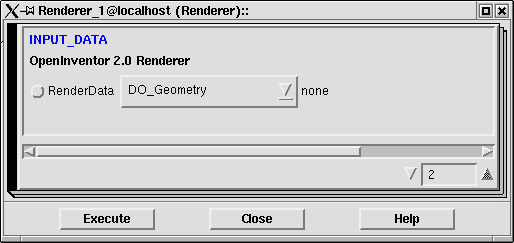
\includegraphics[scale=0.7]{renderer/pict/image2}
   \caption{Renderer Module Setup in the MapEditor}
	\label{fig49}
  \end{center}
 \end{figure}
 \endlatexonly

 

\section{Cooperative Working Modes}

see Chapter 5, COVISE CE, section MasterCtrl, subsection Synchronization

%The COVISE renderer is able to communicate with other renderers in a cooperative
%working session in a master/slave relationship. The communication between
%renderers is done by passing special kinds of messages via the controller.
%That means, no renderer knows anything about the existence of any other renderer.
%For the user the updating of the scene view in the cooperative environment is
%handled transparently. As already mentioned, there is a master/slave relationship
%established in a cooperative session. If the master e.g. translates the camera
%view by dragging the mouse, the view becomes updated on the remote renderer's side. 

%Currently in tight coupled and master/slave relationship the 

%\begin{itemize}
%\item Telepointer
%\item Object transformations
%\item Camera positions
%\item Draw style and draw mode
%\item Picking/editing mode
%\item Background color editing
%\item Switching of fog, antialiasing and axes on/off
%\end{itemize}

%become automatically updated in the other slave renderer windows. Advanced features
%like changing material properties or adding new lights to a scene are merely thought
%for local use and postprocessing of data and therefore not sent to the partners.
%However, the most important thing for cooperative working, that is the placement,
%the orientation of objects and the viewers perspective in respect to the scene,
%are always the same for all partners.
%(Strictly speaking, there is a
%slight difference between "Master/Slave Mode" and "Tight Coupling": "Master/Slave" causes the slave
%renderer to be updated at the end of a move only, whereas "Tight" makes a contiuous update. The two
%possibilities have been introduced due to performance considerations.)



\subsection{Using the Telepointer}

see Chapter 5, COVISE CE, section MasterCtrl, subsection Telepointer

%In addition to the COVISE multimedia support, the renderer introduces the Telepointer.
%The telepointer operates in all directions. If you press the SHIFT key on your
%keyboard, your machine's name will appear at your current mouse position in the
%other renderer's drawing areas. To set the telepointer to another position,
%release the SHIFT key, move the mouse and press SHIFT again at the new position,
%or move the mouse while the SHIFT key is still pressed.

\section{The Renderer's User Interface}

In the following sections the components of the renderer user interface are discussed.

\html{\htmladdimg{pict/general.png}} 
 \latexonly
 \begin{figure}[htp]
  \begin{center}
   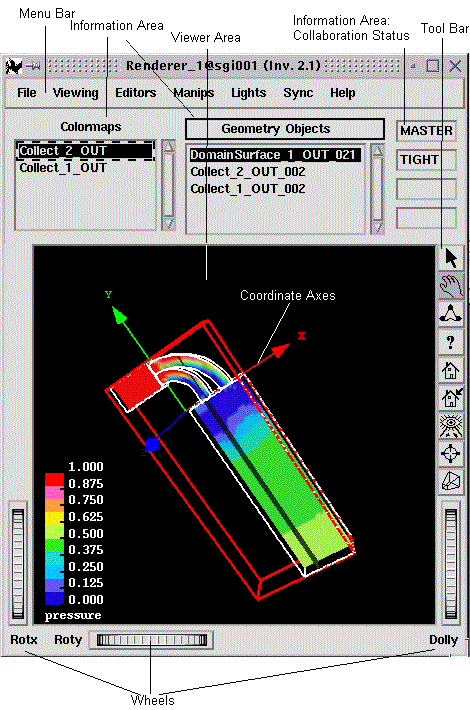
\includegraphics[scale=0.7]{renderer/pict/general}
   \caption{Renderer Main Window Components}
	\label{fig50}
  \end{center}
 \end{figure}
 \endlatexonly

\clearpage

\subsection{The Viewer Area}

In the viewer area objects are displayed and can be manipulated in several ways.
The coordinate axes show the current view orientation.

\subsubsection{Direct Interaction}

Using the mouse buttons in viewing mode affects the camera position, the line of
sight, and the angle of vision in respect to the scene. In the default viewing mode,
the mouse buttons have the functionality as described earlier. In edit (pick)
mode, pressing the left mouse button selects the object under the mouse cursor.
When seeking is enabled by clicking on the seek icon, pressing the left mouse
button starts seeking to the selected point.

% \html{\htmladdimg{pict/image4.png}} 
% \latexonly
% \begin{figure}[htp]
%  \begin{center}
%   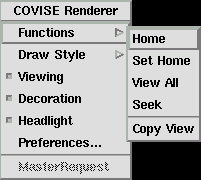
\includegraphics[scale=0.7]{renderer/pict/image4}
%   \caption{The Viewer Popup Menu}
%	\label{fig51}
%  \end{center}
% \end{figure}
% \endlatexonly

 \html{\htmladdimg{pict/popup.png}} 
 \latexonly
 \begin{figure}[htp]
  \begin{center}
   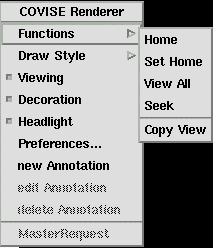
\includegraphics[scale=0.7]{renderer/pict/popup}
   \caption{The Viewer Popup Menu}
	\label{fig51}
  \end{center}
 \end{figure}
 \endlatexonly


\subsubsection{The Viewer Popup Menu}

The popup menu (\ref{fig51}) is activated by clicking the right mouse button while
the mouse pointer is positioned in the viewer area. The popup menu contains
several items and sub menus. These are:

\begin{itemize}
\item {\bf Functions}: The items of this popup sub menu correspond to the icons
on the right side of the viewer area.

\item {\bf Draw Styles}: There are two drawing modes (Still Mode and Move Mode) and seven different drawstyles
for each of these modes, among which the user can choose.   Move Mode is
automatically enabled when interactively moving objects or the camera
using the mouse. The objects may be rendered in a simpler style when
selecting one of the menu items. This is especially useful on slower
machines; thus z-buffering is turned off while rendering in these styles.
The different mode items are:

\begin{itemize}
\item As is
\item Hidden Line
\item No Texture
\item Low Resolution
\item Wireframe
\item Points
\item Bounding box
\end{itemize}

The last three items of the drawstyle sub menu in the viewer popup menu activate
single buffering, double buffering or the switching between single buffering
during manipulation and double buffering otherwise.

% \html{\htmladdimg{pict/image6.png}} 
% \latexonly
% \begin{figure}[htp]
%  \begin{center}
%   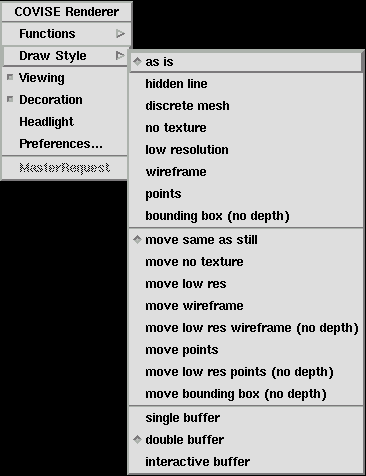
\includegraphics[scale=0.7]{renderer/image6}
%   \caption{Available Drawstyles in the Viewer Popup Menu}
%	\label{fig52}
%  \end{center}
% \end{figure}
% \endlatexonly

 \html{\htmladdimg{pict/drawstyle.png}} 
 \latexonly
 \begin{figure}[htp]
  \begin{center}
   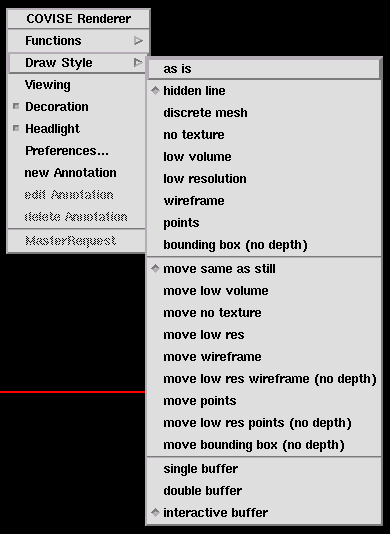
\includegraphics[scale=0.7]{renderer/pict/drawstyle}
   \caption{Available Drawstyles in the Viewer Popup Menu}
	\label{fig52}
  \end{center}
 \end{figure}
 \endlatexonly
 
You can see different viewing modes in  \ref{fig53}, \ref{fig54}, and \ref{fig55}. The
hidden line representation removes all lines which normally could be seen 
shining through in a wireframe representation.

 \html{\htmladdimg{pict/image8.png}} 
 \latexonly
 \begin{figure}[htp]
  \begin{center}
   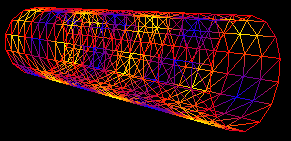
\includegraphics[scale=0.7]{renderer/pict/image8}
   \caption{Wireframe Representation}
	\label{fig53}
  \end{center}
 \end{figure}
 \endlatexonly

 \html{\htmladdimg{pict/image9.png}} 
 \latexonly
 \begin{figure}[htp]
  \begin{center}
   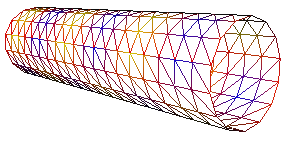
\includegraphics[scale=0.7]{renderer/pict/image9}
   \caption{Hidden Line Representation}
	\label{fig54}
  \end{center}
 \end{figure}
 \endlatexonly

 \html{\htmladdimg{pict/image10.png}} 
 \latexonly
 \begin{figure}[htp]
  \begin{center}
   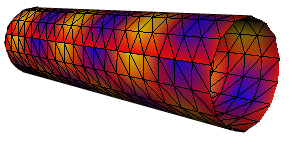
\includegraphics[scale=0.7]{renderer/pict/image10}
   \caption{Discrete Representation}
	\label{fig55}
  \end{center}
 \end{figure}
 \endlatexonly

\clearpage

\item {\bf Viewing}: Toggles between View and Edit (Pick) mode. When picked, a red bounding
box appears surrounding the selected object (\ref{fig56}). 

 \html{\htmladdimg{pict/image11.png}} 
 \latexonly
 \begin{figure}[htp]
  \begin{center}
   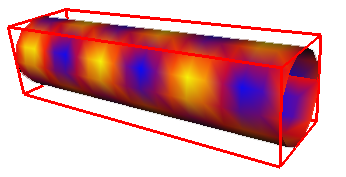
\includegraphics[scale=0.7]{renderer/pict/image11}
   \caption{A Selected (Picked) Object}
	\label{fig56}
  \end{center}
 \end{figure}
 \endlatexonly

When you click on the background in the viewer area the object becomes deselected
again. You can only select one object at a time.

\item {\bf Decoration}: Hides and shows the decoration around the render area. The render area appears a
bit enlarged while decoration is hidden.

\item {\bf Headlight}: Switches the headlight on and off. If you are in PHONG shading mode and no other
lights are active, the objects may become invisible depending on the direction of
the normals on the object surface. It is possible to add more lights to a scene.
This is described later in this chapter.

\item {\bf Preferences}: You can select options from the Preference Sheet:
 \html{\htmladdimg{pict/image12.png}} 
 \latexonly
 \begin{figure}[htp]
  \begin{center}
   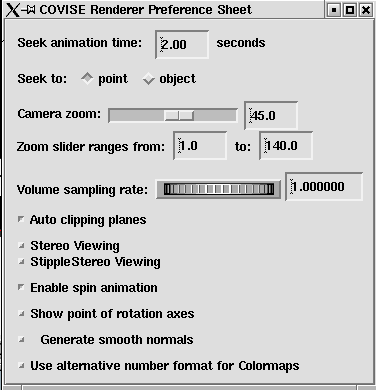
\includegraphics[scale=0.7]{renderer/pict/image12}
   \caption{The Preference Sheet}
	\label{fig57}
  \end{center}
 \end{figure}
 \endlatexonly
\clearpage
 
A menu appears in which defaults for the seek mode, zoom slider bounds, clipping
planes and stereo viewing can be set, or an {\bf alternative number format for colormaps} can
be specified:\newline
This field can be used to specify formats of the numbers along the
color legend. It must be a float format for the "printf" format as
specified in the unix manual pages and should be left-justified.
\begin{verbatim}
Examples: Values 0 0.1 0.2 0.3 0.4 0.5

Format: %-.3f   -->   0.000 0.100 0.200 0.300 0.400 0.500
        %-.2f   -->   0.00 0.10 0.20 0.30 0.40 0.50
\end{verbatim}	
The Volume sample rate thumbwheel is needed for
Volume Rendering (see Appendix).

%When stereo viewing is enabled, a thumb wheel appears, where the stereo offset
%can be adjusted to improve the stereo impression (See "Stereo Viewing Mode" on
%page 58). 

When Spin Animation is enabled, objects can be rotated around in an
animated fashion in viewer mode.


\item {\bf Annotation} (new, edit, delete): With the items of this sub menu (new Annotation / edit Annotation /
delete Annotation) you can add a description to the Renderer image, like "isosurface" in
the figure below.

 \html{\htmladdimg{pict/annotation.png}} 
 \latexonly
 \begin{figure}[htp]
  \begin{center}
   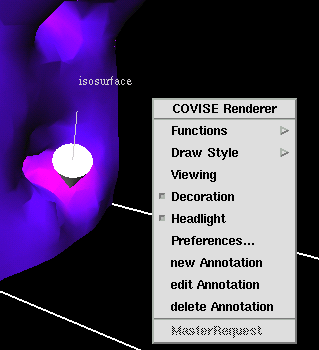
\includegraphics[scale=0.7]{renderer/pict/annotation}
   \caption{Annotion function}
	\label{fig57a}
  \end{center}
 \end{figure}
 \endlatexonly
 
Switch to pick mode and click on the detail you want to explain:
You can now (using a popup with "apply")
\begin{itemize}
\item add a {\bf new Annotation}
\item {\bf edit} an existing {\bf Annotation}
\item {\bf delete} an {\bf Annotation}
\end{itemize}

Please note:
\begin{itemize}
\item Annotations can be saved as part of a map
\item Annotations are "static" - they do not move e.g. with an isosurface if the isovalue is changed
\end{itemize}

\item {\bf MasterRequest}: same function as MasterCtrl in MapEditor

\end{itemize}
\clearpage

\subsubsection{The Decoration Area}

The decoration consists of three thumb wheels for rotating (Rotx, Roty) and
zooming (Dolly) as well as a zoom slider trim (Zoom) and six viewer icons to
the right side of the viewer area. These icons are shortcuts for some of the
viewer pop-up functionality. From top to bottom there are icons for 

\begin{itemize}
\item switching between View and 
\item Edit (Pick) Mode
\item Head Tracking Mode (currently not implemented)
\item invoking the help browser (Help) - not implemented, use help button in menu bar instead
\item resetting camera position to the home position (Home)
\item saving a new home position for the camera view (Set Home)
\item viewing the whole scene (View All)
\item seeking to a certain point of the scene (Seek)
\end{itemize}

\clearpage

\subsection{The Menu Bar}

The menu bar of the renderer window is shown below.

 \html{\htmladdimg{pict/menubar.png}} 
 \latexonly
 \begin{figure}[htp]
  \begin{center}
   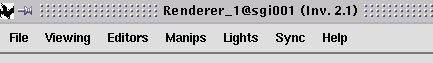
\includegraphics[scale=0.7]{renderer/pict/menubar}
   \caption{Renderer Menubar}
	\label{fig58}
  \end{center}
 \end{figure}
 \endlatexonly

\subsubsection{File Menu}

 \html{\htmladdimg{pict/image13.png}} 
 \latexonly
 \begin{figure}[htp]
  \begin{center}
   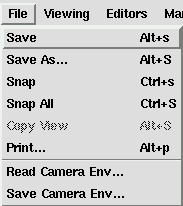
\includegraphics[scale=0.7]{renderer/pict/image13}
   \caption{The File Menu}
	\label{fig59}
  \end{center}
 \end{figure}
 \endlatexonly

\begin{itemize}
\item {\bf Save}: The current objects are saved in Inventor 3D format. Programs reading this format
like IRIS Explorer or IRIS Showcase can load this objects and allow further usage
and postprocessing of the 3D data.

\item {\bf Save as}: Save the whole scene. A file selector box appears where directory and file name
can be selected.

\item {\bf Snap}: Take a snapshot of the viewer area. Format of the snapshot files is .tiff
(changed with Rel. 5.2.3). Creates an error dialog if offscreen rendering
is not possible due to low colordepth. Offscreen rendering requires at
least a 24bit true color. Same applies to Snap all.

\item {\bf Snap all}: Take a series of snapshots of the viewer area.\newline
You can use this series of snapshots in order to {\bf generate a simple
movie}.\newline
Example on SGI: call {\bf 'mediaconvert'} and fill in the entries as shon below

\html{\htmladdimgpict{pict/mediaconvert.png}} 
 \latexonly
 \begin{figure}[htp]
  \begin{center}
   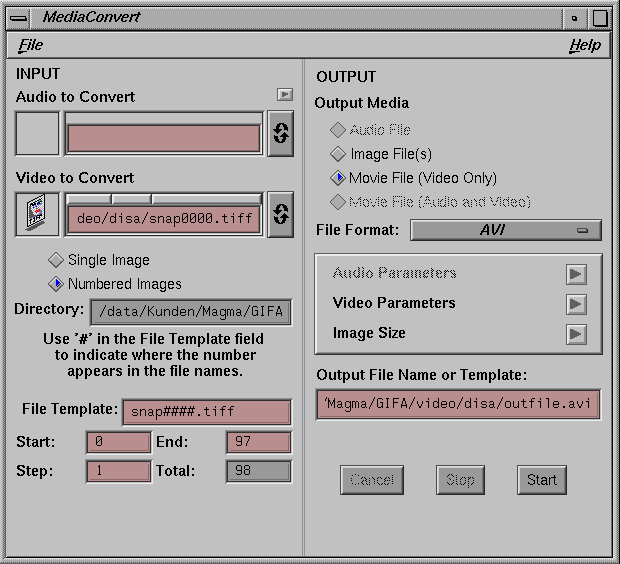
\includegraphics[scale=0.6]{renderer/pict/mediaconvert}
   \caption{MediaConvert - Movie on SGI}
	\label{fig59a}
  \end{center}
 \end{figure}
 \endlatexonly
\clearpage

\item {\bf Copy View}: The currently selected object is copied to a buffer from which other programs
like IRIS Showcase can directly paste the 3D object into their application. 

\item {\bf Print}: It is possible to save the currently visible scene in an Postscript file or to
send the postscript output directly to a printer. The available printers are
listed below in the printer list. The output quality and print size in inches
can be adjusted The page format can be chosen between landscape or portrait.

 \html{\htmladdimg{pict/image14.png}} 
 \latexonly
 \begin{figure}[htp]
  \begin{center}
   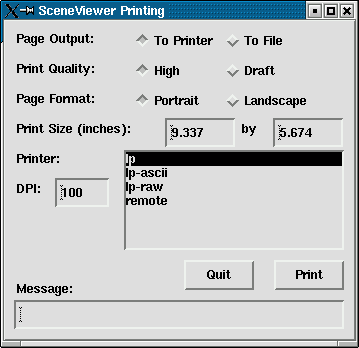
\includegraphics[scale=0.7]{renderer/pict/image14}
   \caption{The Printing Menu}
	\label{fig60}
  \end{center}
 \end{figure}
 \endlatexonly

\item{\bf Read/Save Camera Env...}: Restore/Save the camera environment

\end{itemize}
\clearpage

\subsubsection{Viewing menu}

The viewing menu is shown in \ref{fig61}.

\begin{itemize}
\item {\bf Pick/Edit}:

By default the renderer is in the View mode. The viewer uses a virtual
trackball to rotate the scene graph around the point of interest. If you want
to change the view of a scene but a specific object in respect to other objects,
you have to switch from the View mode to Pick/Edit mode. In Edit mode the
outlined hand cursor changes to an arrow shape cursor. If you click on an object
with the left mouse button, the object becomes selected and highlighted by a
red wireframe box which now surrounds the object. You can select only one object
at a time. If you have opened any editors or enabled manipulators, these will
be attached to the selected target object for further editing. If you switch
between objects by clicking on a different object all manipulators and editors
automatically become attached to this object.

 \html{\htmladdimg{pict/image15.png}} 
 \latexonly
 \begin{figure}[htp]
  \begin{center}
   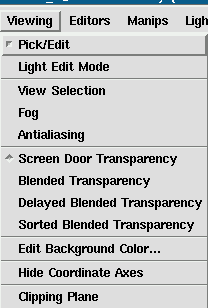
\includegraphics[scale=0.7]{renderer/pict/image15}
   \caption{The Viewing Menu}
	\label{fig61}
  \end{center}
 \end{figure}
 \endlatexonly
\clearpage

\item {\bf Light Edit Mode}:

Enabling this mode lets you interactively edit the current visible light sources
in the scene by using the mouse. 

\item {\bf Fog}:

This item affects the environment of a scene to simulate various atmospheric
effects such as fog, haze, pollution and smoke which are grouped under the term fog.

\item {\bf Anti-aliasing}:

 This technique is useful to eliminate or reduce jagged lines and make objects
 drawn on the screen look smooth. Enabling this item reduces drawing speed.

\item {\bf Screen Door Transparency}:

This and the next three items affect the transparency quality level. Screen
door transparency is the default and the only supported mode on some machines.
For transparency details refer to the editor's section. Screen door
transparency uses GL patterns for achieving the transparency effect.

\item {\bf Blended Transparency}:

 uses GL alpha blending.

\item {\bf Delayed Blended Transparency}:

 uses GL alpha blending, opaque objects are rendered first, then transparent objects.

\item {\bf Sorted Blended Transparency}:

uses GL alpha blending, opaque objects are drawn first, then transparent objects.
Additionally the objects are sorted by their distance from the camera and are
drawn from back to the front.



\item {\bf Edit Background Color}:

Invokes a color editor for changing the background color of the render area (default is black).

\item {\bf Hide Coordinate Axes}:

Toggles between hiding and showing the three coordinate axes. The axes are on by default.

\item {\bf Clipping Plane}: Cut Geometry

\end{itemize}
\clearpage

\subsubsection{Editors menu}

 \html{\htmladdimg{pict/editors.png}} 
 \latexonly
 \begin{figure}[htp]
  \begin{center}
   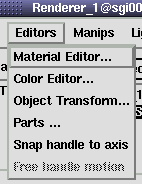
\includegraphics[scale=0.7]{renderer/pict/editors}
   \caption{Editors Menu}
	\label{fig62}
  \end{center}
 \end{figure}
 \endlatexonly

\begin{itemize}
\item {\bf Material Editor}:

The material editor is used for customizing objects by interactively changing
values for ambient, diffuse, specular, transparent, emissive and shininess
elements and immediately seeing the effects of these changes.

 \html{\htmladdimg{pict/image16.png}} 
 \latexonly
 \begin{figure}[htp]
  \begin{center}
   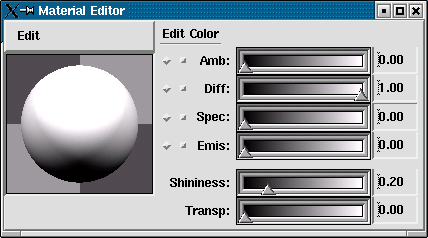
\includegraphics[scale=0.7]{renderer/pict/image16}
   \caption{The Material Editor}
	\label{fig63}
  \end{center}
 \end{figure}
 \endlatexonly



The diffuse color is the object's base color specified in the color array of
the renderer geometry input data objects. If no colors are specified, the color
of each vertex of the object is set to RGB [1.0 1.0 1.0] default. Editing the
diffuse color of those objects affects all vertices of the object, thus the
whole object changes its color. If one color is specified for the whole object
(color binding OVERALL) all vertices of the object are colored according to
this value. If you edit the diffuse color of these objects, also all vertices
are affected by color changes. If vertex based objects such as polygons or
lines with colors attached per vertex (color binding PER\_VERTEX) or per face
(binding PER\_FACE) are present, only the first vertex is affected by changes
of the diffuse color field, therefore editing the diffuse color of those
objects is not very useful. The next items affect the whole object in any
case. The Ambient Color is the reflected color of an object in response to
the ambient lighting in the scene. The default value for this field is [0.2 0.2 0.2].
The Emissive Color is the light caused by self illuminating objects.
The default for this field is [0.0 0.0 0.0], which means the object
is emitting no light. The degree of shininess of an object's surface
is for e.g. achieving metallic effects on the surface of an airplane
wing. The value ranges from 0.0 (default) for a diffuse surface with
no shininess to 1.0 for a highly polished surface. Let us assume there
are two objects present by one object covering the other, where one
cannot see the covered object. By adjusting the Transparency Level of
the covering object you can see either both (values larger than 0.0)
or only the previously covered object (value 1.0).

\item {\bf Color Editor}:

The color editor lets you interactively change the color properties of an
object, a light source or the background color of the render area. You can
set RGB or HSV values or pick a color directly from the color wheel. By
selecting Manual from the edit menu bar item you can prevent changes being
reflected immediately in the object until you are ready. Use the two color
squares to test new colors and store the previous one. By clicking on the
three pads beneath the squares, you can switch back and forth between colors.
The new color is always on the left and the previous color on the right.
You can send the new color to the right square, or the old color to the
left square. RGB values range from 0.0 to 1.0 for the red, green and blue
color component, where [0.0 0.0 0.0] is black and [1.0 1.0 1.0] is white.

 \html{\htmladdimg{pict/image17.png}} 
 \latexonly
 \begin{figure}[htp]
  \begin{center}
   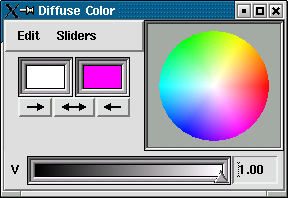
\includegraphics[scale=0.7]{renderer/pict/image17}
   \caption{The Color Editor}
	\label{fig63a}
  \end{center}
 \end{figure}
 \endlatexonly

\item {\bf Object Transform}:

Transform sliders are useful to change the position of objects in respect
to each other or to scale an object to make it appear larger or smaller on
the screen. If you click on an item in the transform slider set sub menus
appear in which you can do the desired editing operations by adjusting
sliders with the mouse or typing exact values using input fields. There
are three different widget layout styles available, simply click on Style
in the slider menu. Note that the changes only affect the currently
selected object in the scene. Translation changes the position of an
object in the scene. Scale changes the size of an object. Rotation
changes the orientation of the object in the scene. Scale Orientation
changes the orientation for scale operations. Center changes the center
around which rotations take place.

 \html{\htmladdimg{pict/image18.png}} 
 \latexonly
 \begin{figure}[htp]
  \begin{center}
   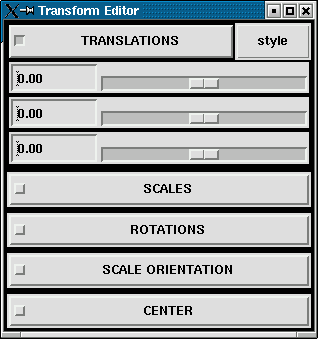
\includegraphics[scale=0.7]{renderer/pict/image18}              
   \caption{The Transform Editor}
	\label{fig64}
  \end{center}
 \end{figure}
 \endlatexonly

\clearpage

\item {\bf Part Editor}:

If the geometry objects displayed by the Renderer can be identified (in case of modules 
using finite elements) you can use the {\bf COVISE Part Editor} to select which parts of 
the geometry will become visible or invisible and, optionally, which part is fixed 
during movements.

 \html{\htmladdimg{pict/partedit.png}} 
 \latexonly
 \begin{figure}[htp]
  \begin{center}
   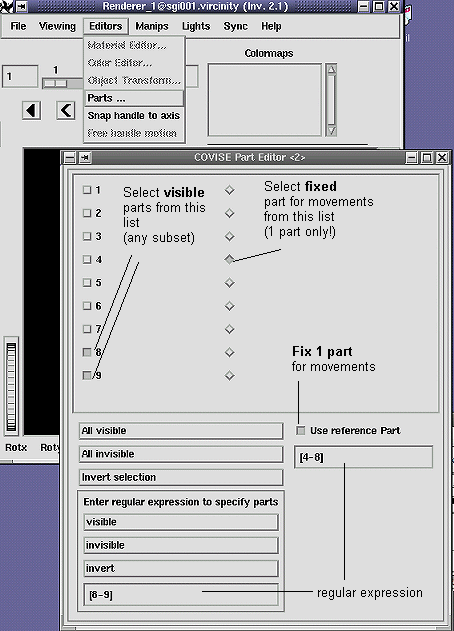
\includegraphics[scale=0.7]{renderer/pict/partedit}
   \caption{Part Editor}
	\label{fig65}
  \end{center}
 \end{figure}
 \endlatexonly

The {\bf left side} of the Part Editor window provides the functions to select which parts 
are {\bf visible}; you have 3 possibilities:
\begin{itemize}
\item Select any subset of parts out of the selection list (toggle switches,any subset)
\item Set all parts visible/invisible or invert your selection
\item Specify the subset of parts by a regular expression and press RETURN
\end{itemize}

On the {\bf right side} you can (optionally) select a {\bf reference part} that will be 
{\bf fixed } during movements; to specify this reference part you can use 2 possibilities:
\begin{itemize}
\item Select this part from the list (toggle switches, 1 part only)
\item Specify a regular expression and press RETURN; the first part matching the 
regular expression is fixed.
\end{itemize}

\clearpage

\item{\bf Interactors (Snap/Free handle)}:

The last two options of the Editors menu item have been added to select options for an 
{\bf Interactor}. If you want to move e.g. a Cutting Surface,
you can attach an interactor to it. An interactor attached to a point of
a Cutting Surface consists of

\begin{itemize}
\item a {\bf tangential plane} (reduced to a square) at that point
\item a {\bf normal} at that point
\end{itemize}
(see example below)

\html{\htmladdimg{pict/interactor.png}} 
 \latexonly
 \begin{figure}[htp]
  \begin{center}
   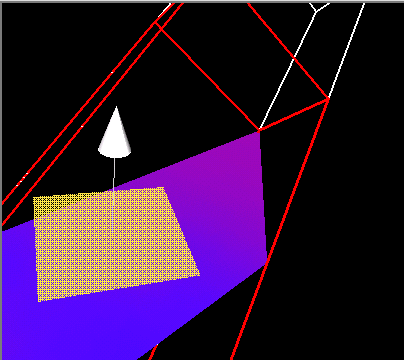
\includegraphics[scale=0.7]{renderer/pict/interactor}
   \caption{Interactor}
	\label{fig65a}
  \end{center}
 \end{figure}
 \endlatexonly
 
You attach an interactor by clicking on a point of the Cutting Surface.

Note: You must be in pick mode and select (click on) the Cutting Surface before you 
can attach an interactor

You can
\begin{itemize}
\item {\bf rotate} the Cutting Surface by using the normal (arrow) as a handle 
\item {\bf translate} the Cutting Surface by pulling the plane
\end{itemize}

You use the option
\begin{itemize}
\item {\bf Snap handle to axis} in order to in order to enable ... 
\item {\bf Free handle motion} in order to disable the orientation of 
CuttingSurfaces normal to coordinate axis
\end{itemize}

\end{itemize}
\clearpage

\subsubsection{Manips menu}

Manipulators are used for direct manipulation of a certain object, like
the editors explained in the last section. 

 \html{\htmladdimg{pict/image19.png}} 
 \latexonly
 \begin{figure}[htp]
  \begin{center}
   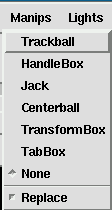
\includegraphics[scale=0.7]{renderer/pict/image19}
   \caption{The Manips Menu}
	\label{fig66}
  \end{center}
 \end{figure}
 \endlatexonly

This way of manipulation is more direct than using editors, but less precise
than using the sliders. To attach a manipulator to an object, switch to the
picking mode and select a manipulator type in the Manips Menu  shown in \ref{fig66}.

Now click on the desired object. The manipulator appears and surrounds
the object. There are different manipulators to transform, rotate, scale,
and move an object in the viewer. 

\begin{itemize}
\item {\bf Trackball}:

This manipulator is for rotating and scaling an object. It appears as a
transparent sphere around the selected object.

 \html{\htmladdimg{pict/image20.png}} 
 \latexonly
 \begin{figure}[htp]
  \begin{center}
   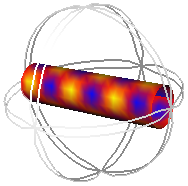
\includegraphics[scale=0.7]{renderer/pict/image20}
   \caption{Object with Trackball Manipulator Attached}
	\label{fig67}
  \end{center}
 \end{figure}
 \endlatexonly
\item {\bf Handle Box}: This inserts a transparent cube into the scene that allows the user to
scale and translate the object by moving the mouse in various ways.
Use the SHIFT and ALT keys with the left mouse button to achieve specific
effects for both the trackball and the handlebox manipulator. (see \ref{fig68})

\item {\bf Jack}: The object can be zoomed and rotated.

\item {\bf Centerball}: Is for moving the center point of rotation for an object. Afterwards
the object can be rotated around the new rotation point.

\item {\bf TransformBox}: This manipulator is for transforming the selected object. 

\item {\bf TabBox}: This lets you scale an object by doing a click-drag-release motion with
the mouse after clicking on the green control points.

\item {\bf None}: This is the default. If an object gets picked, no manipulator is attached to the object.

\item {\bf Replace}: If a different manipulator is selected from the list the currently active
manipulator is either replaced or stays attached. 

 \html{\htmladdimg{pict/image21.png}} 
 \latexonly
 \begin{figure}[htp]
  \begin{center}
   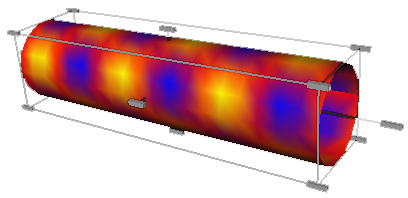
\includegraphics[scale=0.7]{renderer/pict/image21}
   \caption{Tube Surrounded by a Handlebox Manipulator}
	\label{fig68}
  \end{center}
 \end{figure}
 \endlatexonly
\end{itemize}

\clearpage


\subsubsection{Lights menu}

The lights menu is for creating, editing, and removing light sources
in an object scene. This is a feature used for changing the appearance
of an object by changing its illumination. Light information is
currently not sent to other renderers in a cooperative working environment.
Each entry in the menu is explained now in detail.

 \html{\htmladdimg{pict/image22.png}} 
 \latexonly
 \begin{figure}[htp]
  \begin{center}
   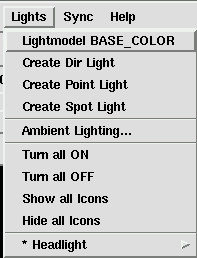
\includegraphics[scale=0.7]{renderer/pict/image22}
   \caption{The Lights Menu}
	\label{fig69}
  \end{center}
 \end{figure}
 \endlatexonly

\begin{itemize}
\item {\bf Lightmodel BASE\_COLOR}: Each object has its own base color also called diffuse color. If no
colors are specified, the objects are colored white over all faces
or vertices. When the base color model is enabled (the default), all
objects are rendered by taking only their diffuse color into account.
If it is disabled all objects are PHONG shaded. The PHONG lighting
model takes into account all light sources in the scene and the object's
surface orientation (the normals on faces or vertices) with respect to
the lights to generate a realistic smooth shaded 3D appearance of an
object. Scientists often prefer to see only the real colors defined
for the object without shading effects, so switching between the two
modes is introduced here.
\item {\bf Create Dir Light}: This creates a light which illuminates uniformly along a particular direction.

\item {\bf Create Point Light}: A point light, like a star, radiates light equally in all directions
from a given location in 3D space.

\item {\bf Create Spot Light}: A spot light illuminates from a point in space along a primary direction.
Its illumination is a cone of light diverging from the light's position.
This feature is hardware dependent. If not supported, a spotlight appears
as a point light.

 \html{\htmladdimg{pict/image23.png}} 
 \latexonly
 \begin{figure}[htp]
  \begin{center}
   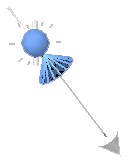
\includegraphics[scale=0.7]{renderer/pict/image23}
   \caption{The Spot Light Icon}
	\label{fig69}
  \end{center}
 \end{figure}
 \endlatexonly

\item {\bf Ambient Lighting}: This is used for the PHONG lighting mode, it lets you edit the ambient
ligthing in the scene.

\item {\bf Turn all ON}: Turns all currently defined light sources on.

\item {\bf Turn all OFF}: Turns all currently defined light sources off.

\item {\bf Show all Icons}: Shows the icons of the currently defined light sources.

\item {\bf Hide all Icons}: Hides the icons of the currently defined light sources.

\item {\bf Headlight}: This is the default light. A sub menu lets you edit the color of this
light or removing it from the scene. The icon for the headlight is turned off by default. If you create new lights, new entries will appear below. 

\item {\bf New lights}: are shown by placing the light icon at a default position in the scene.
These lights can be edited interactively with the mouse after turning
on the Light editing mode. To edit the properties of a light you can
also select Edit from the sub menu of the Headlight item.
The edit window appears, displaying the light you have selected.
You can change the intensity of the light emanating from the source
by moving the intensity slider. You can also adjust the angle at which
the light shines on the object by clicking on the directional arrow and
changing its position in the window. Editing the color of the light
brings up the color editor. 

 \html{\htmladdimg{pict/image24.png}} 
 \latexonly
 \begin{figure}[htp]
  \begin{center}
   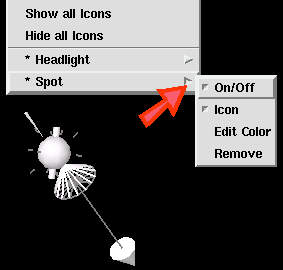
\includegraphics[scale=0.7]{renderer/pict/image24}
   \caption{New Light Entries}
	\label{fig70}
  \end{center}
 \end{figure}
 \endlatexonly
 
 \html{\htmladdimg{pict/image25.png}} 
 \latexonly
 \begin{figure}[htp]
  \begin{center}
   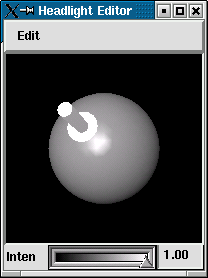
\includegraphics[scale=0.7]{renderer/pict/image25}
   \caption{The Light Editor Menu}
	\label{fig71}
  \end{center}
 \end{figure}
 \endlatexonly

\end{itemize}
\clearpage

\subsubsection{Sync menu}

\html{\htmladdimg{pict/image26.png}} 
 \latexonly
 \begin{figure}[htp]
  \begin{center}
   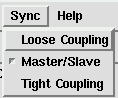
\includegraphics[scale=0.7]{renderer/pict/image26}
   \caption{The Sync Menu}
	\label{fig72}
  \end{center}
 \end{figure}
 \endlatexonly
 
see Chapter 5, COVISE CE, section MasterCtrl, subsection Synchronization

%relationship has been established between the partners of a working session.
%From the renderer's point of view this means that there is only one
%partner who has all of the interaction facilities. This is often
%inconvenient. Assume other partners want to save a certain scene or
%object without having to ask the master to take over control for this
%single operation.

%COVISE offers three degrees of coupling:

%\begin{description}
%\item[Loose Coupling] mode has been introduced as an addition to the master/slave and tight
%coupling mode.
%If the master enables this mode all partners have the same interaction
%facilities as the master. Camera positions and object transformations
%are no longer sent to other renderers. Only the master has the ability
%to switch between the two modes. If the mode is set back to master/slave
%all manipulators and editors become detached and invisible and the menu
%bar is set to insensitive in the slave renderers. Additionally, the
%scene is updated according to the view in the master renderer.  
%\item[Master/Slave] Slave Renderers controlled by Master - update at the end of a move 
%operation. This is the {\bf default} cooperative mode.
%\item[Tight Coupling] Slave Renderers controlled by Master - continuous update. 

% \html{\htmladdimg{pict/image26.png}} 
% \latexonly
% \begin{figure}[htp]
%  \begin{center}
%   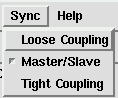
\includegraphics[scale=0.7]{renderer/pict/image26}
%   \caption{The Sync Menu}
%	\label{fig72}
%  \end{center}
% \end{figure}
% \endlatexonly

%\end{description}

\subsubsection{Help}

Pressing Help provides you online help for the Renderer - but you can easily branch e.g. to help for
MapEditor or Modules. 

\clearpage

\subsection{The Information Area}

 \html{\htmladdimg{pict/general.png}} 
 \latexonly
 \begin{figure}[htp]
  \begin{center}
   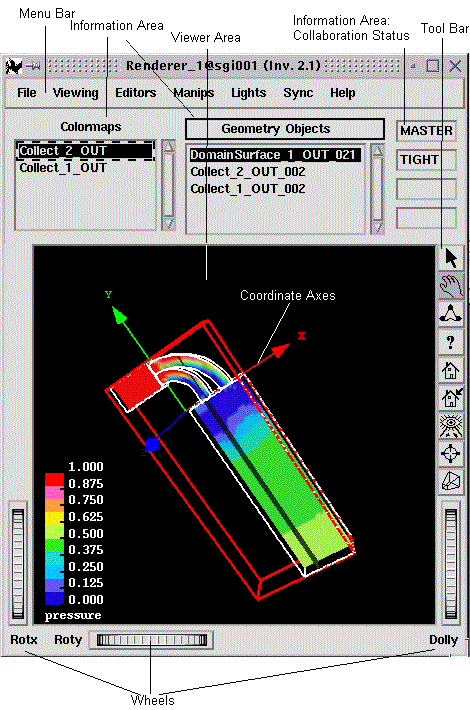
\includegraphics[scale=0.7]{renderer/pict/general}
   \caption{Information Area of the Renderer}
	\label{fig73}
  \end{center}
 \end{figure}
 \endlatexonly

On the left side of the information area, the list of currently displayed geometry objects is shown
(together with the colormaps used).

 \html{\htmladdimg{pict/image28.png}} 
 \latexonly
 \begin{figure}[htp]
  \begin{center}
   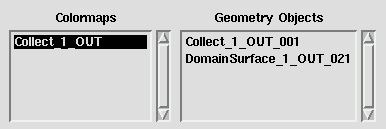
\includegraphics[scale=0.7]{renderer/pict/image28}
   \caption{List of Current Geometry Objects and Color Maps}
	\label{fig74}
  \end{center}
 \end{figure}
 \endlatexonly
 
If you click on a certain object in the render area the name of the object gets highlighted in the object list. It is also possible to select an object in the render area by clicking on it's name in the object list. The red bounding box appears around the selected object in the render area to highlight the selection.
Thus, similar objects can be distinguished by their unique name.


On the right side of the information area there are four lines; the first two display the
collaboration status of the renderer:

\begin{itemize}
\item {\bf Interaction Mode}: Shows whether the renderer is master or slave.

\item {\bf Synchronization}: Tells whether tight, master/slave (=SYNC), or loose coupling is enabled between the renderers in the environment.

\item {\bf Rendering State}: - obsolete, not used

\item {\bf Rendering Time}: - obsolete, not used

\end{itemize}


\section{Using Spaceball and Spacemouse}

% commented following image - logitec no longer present in updated version

% \html{\htmladdimg{pict/image12.png}} 
% \latexonly
% \begin{figure}[htp]
%  \begin{center}
%   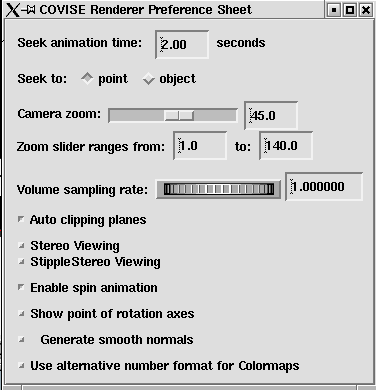
\includegraphics[scale=0.7]{renderer/pict/image12}
%   \caption{CrystalEyes Shutter Glasses, Logitech Ultra Sonic Transmitter and Spacemouse}
%	\label{fig575}
%  \end{center}
% \end{figure}
% \endlatexonly

If the Spaceball or the DLR Spacemouse is connected to your workstation, you are able to manipulate the geometry objects in 3D space in a six degrees of freedom fashion. The device should beep two times at renderer startup time when initialization of the device was successful. To move an object around select the object in picking mode. The device is now attached to the selected object. Some of the device buttons provide some additional functionality:

\begin{itemize}
\item Button 1: Disable/enable rotation
\item Button 2: Disable/enable translation
\item Button *: Set home selected object
\item Button 3: Set home all objects
\end{itemize}

If no object is selected, the spacemouse changes the viewpoint in respect
to the scene by changing the current camera position. 

\section{Stereo Viewing Mode}


 \html{\htmladdimg{pict/image29.png}} 
 \latexonly
 \begin{figure}[htp]
  \begin{center}
   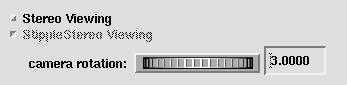
\includegraphics[scale=0.7]{renderer/pict/image29}
   \caption{Stereo mode in the preference sheet}
	\label{fig76}
  \end{center}
 \end{figure}
 \endlatexonly
Some platforms support stereo in a window viewing. Stereo viewing is enabled
by choosing Stereo Viewing in the renderer's preference sheet. You return to
the default mode by deselecting Stereo Viewing in the preference sheet or
typing in a shell window: 

/usr/gfx/setmon -n 72HZ
or
/usr/gfx/setmon -n 60HZ
depending on the type of monitor attached. 

\section{Head Tracking Mode}

currently not implemented

%When a Logitech Head Tracking Device with CrystalEyes shutter glasses is
%connected to a serial port, the visualized data  can be investigated by
%moving  your head. By turning the head, objects can be seen from a different
%angle and by moving the head forward or backward, objects can be seen closer
%or farther. Thus, it is possible to see object from different sides or "fly"
%through a data set. In conjunction with stereo viewing  a much more immersive
%impression is provided to the user which can be helpful in many 3D scientific
%visualization cases. The serial port can be adjusted in the preferences menu.
%It is also possible to use a Polhemus Fastrak tracking device for position
%and orientation detection.

%\section{Performance Considerations in a Cooperative Session}

%Particularly for performance reasons, it is advantageous to know little
%about what is going on behind the scenes when the mouse is moved around
%in the viewer area, especially when working with the master renderer in
%the environment.

%\subsection{Updating the Telepointer}

%The telepointer is operating in all directions. If you press the SHIFT
%key on your keyboard, your machine's name will appear at your current
%mouse position in the other renderer's drawing areas. To reposition the
%telepointer to another position, release the SHIFT key, move the mouse
%and press SHIFT again at the new position, or move the mouse while the
%SHIFT key is still pressed. The difference here is, that in the second
%case the new mouse position is sent over the network very often.

%\subsection{Updating the Head Tracker}

%In head tracking mode, the current tracking update rate can be adjusted
%by the thumbwheel in the viewer preference sheet. A lower update rate
%produces less network traffic. The default tracking rate is currently
%0.1sec. The ideal tracking rate depends heavily on the scene complexity
%and hardware platform used. Also note that the others partner's graphics
%hardware might be not able to render at your locally available graphics
%speed. If you want the head tracking to have only local effect, change
%to loose coupling in the sync menu of the renderer's menu bar. When you
%switch back to tight coupling later on, the screens become automatically
%updated and synchronized again.






    
%\subsubsection{Direct Manipulation}

%Normally, new positional information is only sent, when the master
%releases the mouse button in the viewer area. 

%\subsubsection{Using the Decoration Around the Viewer Area}

%The same is true for the thumb wheels and the slider around the
%viewer. When you release the mouse button information is sent over
%the network. 

%\subsubsection{Using Sliders}

%As far as the sliders in the transform editor are concerned, the situation
%is somewhat different. If you are using the transform sliders by pressing
%the mouse button and moving back and forth, every little movement will
%directly go over the network. If you want to avoid this, click on the
%slider once at the desired position or use the input line. Note that
%renderers running on machines without advanced graphics hardware can
%manually change the scene drawstyle changed to wireframe or points for
%locally doing extensive editing operations. This especially applies to
%the master/slave mode.

%\subsection{System Requirements}

%The COVISE renderer is based on the OpenInventor high level object oriented 
%graphics toolkit developed by Silicon Graphics. OpenInventor itself uses 
%OpenGL, the 3D graphics standard as its rendering interface.

%SGI Systems ship with OpenInventor 2.1 and OpenGL 1.2, there are no
%additional requirements.

%The Rendering speed can vary significantly, depending on the graphics
%adaptor and the quality of the OpenGL implementation. Currently we support SGI, HP and Linux platforms.
%Spacemouse/Spaceball as input device is currently only supported in the SGI
%version.


%Another thing regarding OpenInventor has to be mentioned: On SGI we currently
%support three different Inventor releases: 1.1, 2.0 and 2.1.2. Depending on
%the eoe subsystem installed on your machine there should exist a link from
%one of these renderers (Renderer11,Renderer20,Renderer21) to a module called renderer. 

